Because of the limited amount of discrete commands MusEEG is able to send, it may be helpful for users to control higher level musical events (such as chords, phrases, drum beats, or pre-recorded samples) instead of singular notes. The SuperCollider programming language facilitates the creation of such objects, and may act as a dedicated musical server that responds to OSC commands sent from MusEEG. 

\section{OSCdefs}
\begin{figure}[htbp]
	\centering
		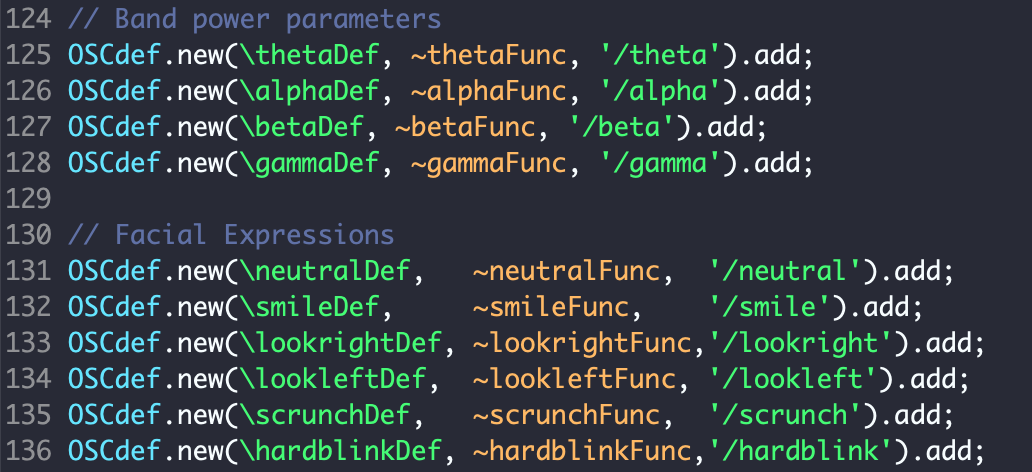
\includegraphics[width=1\columnwidth]{OSCdefs.png}
	\caption{OSCdefs for MusEEG in SuperCollider }
	\label{fig:oscdefs}
\end{figure}

OSCdefs are SuperCollider objects that execute a callback function when a specific OSC message is received. In (Figure~\ref{fig:oscdefs}), a distinct callback function is assigned to each facial expression and band power message, allowing for different facial expressions to send control commands to user-specified musical objects. 


\section{Using SuperCollider as a MIDI server}
SuperCollider's innately friendly MIDI API makes it a more favorable option for programming MIDI patterns than Python. Because of this, MusEEG's MIDI interface  (Figure~\ref{fig:midi-menu}) simply sends OSC messages containing information regarding the chord chosen and some additional control paremeters: arpeggiation, number of repeats, chord duration, and note scrambling. On the other hand, a SuperCollider script takes care of receiving the OSC messages and creating the specified MIDI messages. 

The playChord function (Figure~\ref{fig:playchord}) allows for MIDI messages to be sent in a quantized manner, allowing asynchronously performed facial expressions to have a synchronous effect on the music being performed, and thus rendering a more accessible work flow. 

\begin{figure}[h!]
	\centering
		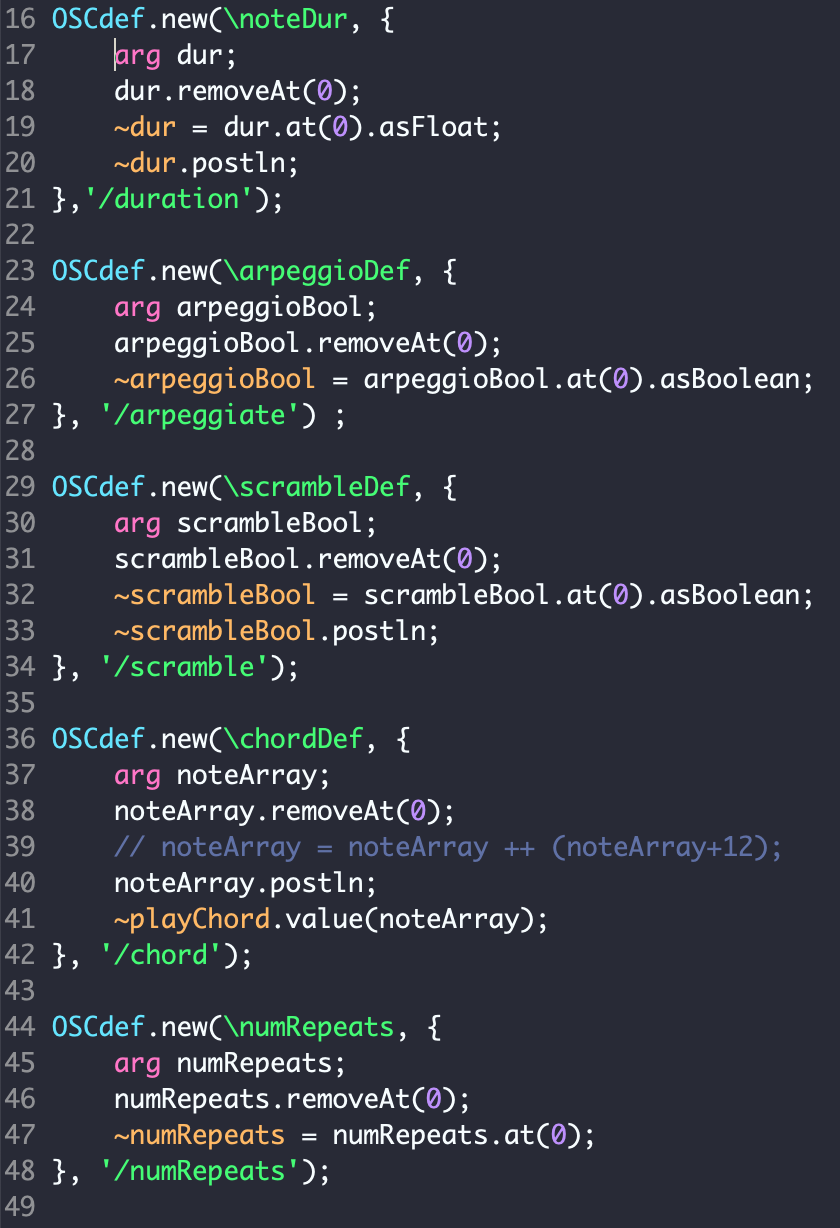
\includegraphics[width=0.5\columnwidth]{midi-oscdefs.png}
	\caption{OSCdefs for MusEEG MIDI}
	\label{fig:midi-oscdefs}
\end{figure}

\begin{figure}[h!]
	\centering
		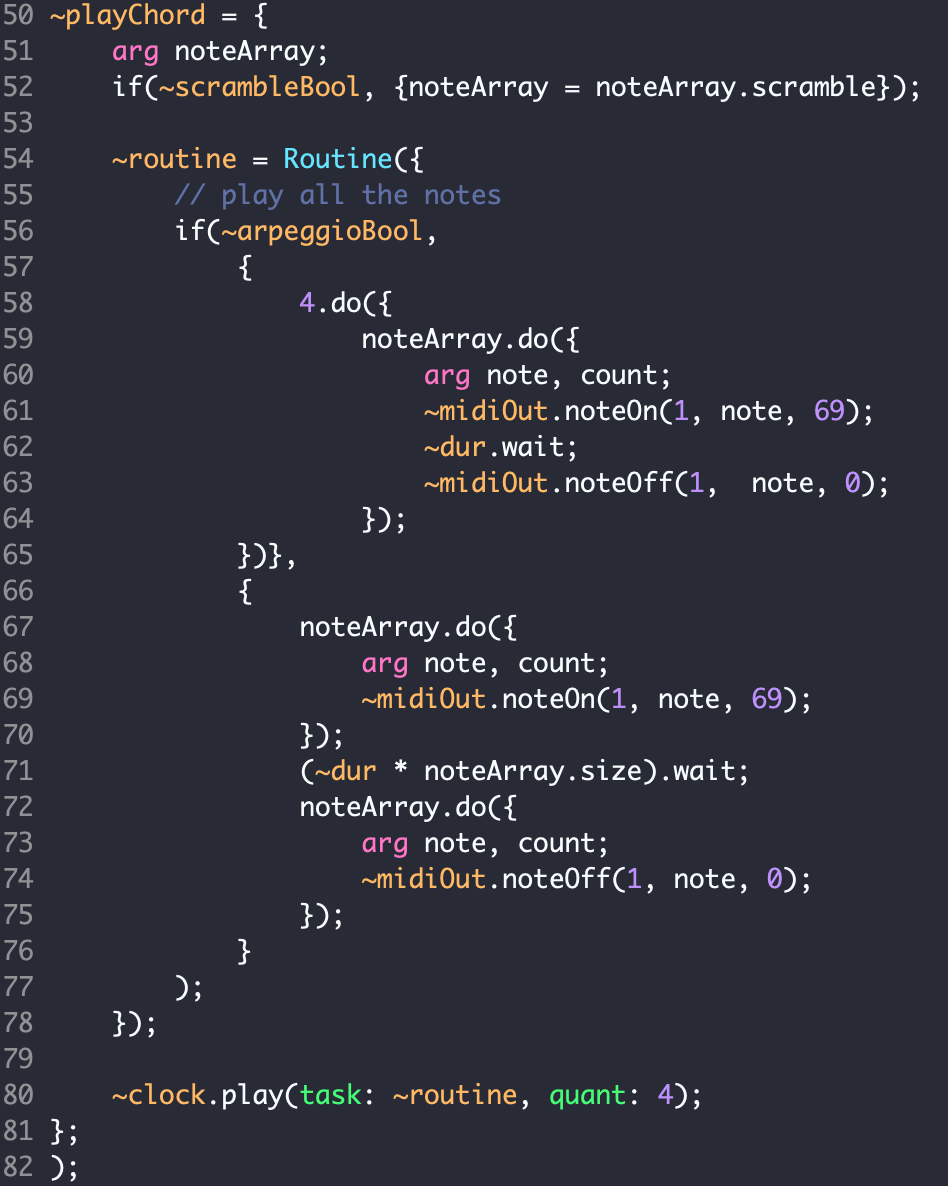
\includegraphics[width=1\columnwidth]{playchord.png}
	\caption{MIDI performance Routine}
	\label{fig:playchord}
\end{figure}

\pagebreak



\section{The Pattern System}

SuperCollider's pattern system provides a simple way of sequencing synthesizer sounds. The MusEEG package includes two examples that demonstrate ways SuperCollider's pattern system may be used in conjunction with MusEEG to control higher level musical events. 

\subsection{A Simple Drum Sequencer}

\begin{figure}[htbp]
	\centering
		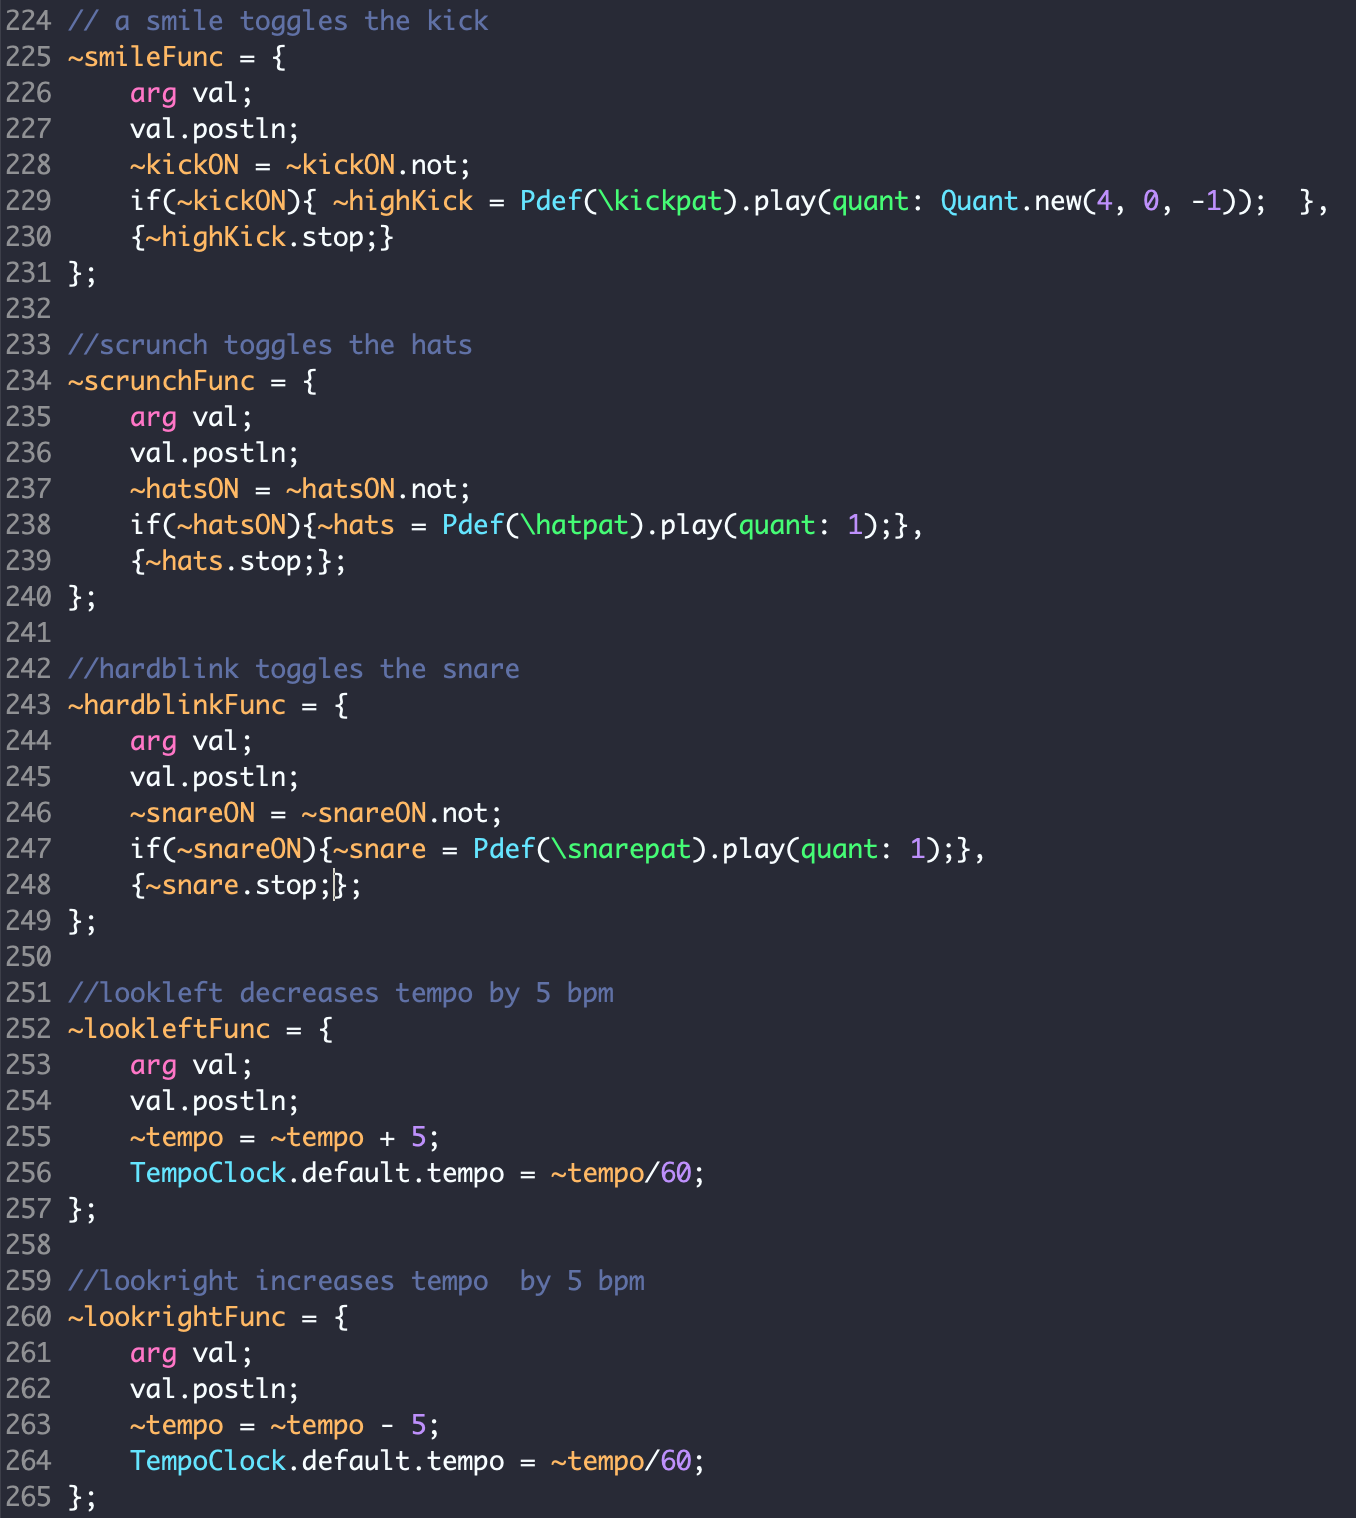
\includegraphics[width=1\columnwidth]{drumsequencer.png}
	\caption{Facial Expression Controls for Drum Sequencer}
	\label{fig:drumsequencer}
\end{figure}

(Figure~\ref{fig:oscdefs}) shows the facial expression callback functions for a drum sequencer pattern in SuperCollider. In this example, the following facial expression controls are enabled:
\begin{itemize}
\item A smile expression toggles a kick drum sound in a drumbeat. 
\item A scrunch expression toggles a hi-hat drum sound in a drumbeat. 
\item A hard blink expression toggles a snare drum sound in a drumbeat. 
\item A look left expression decreases the beat tempo by 5 bpm. 
\item A look right expression increases the beat tempo by 5 bpm.
\end{itemize}

\pagebreak

\subsection{A Generative Arpeggio Pattern}
\begin{figure}[htbp]
	\centering
		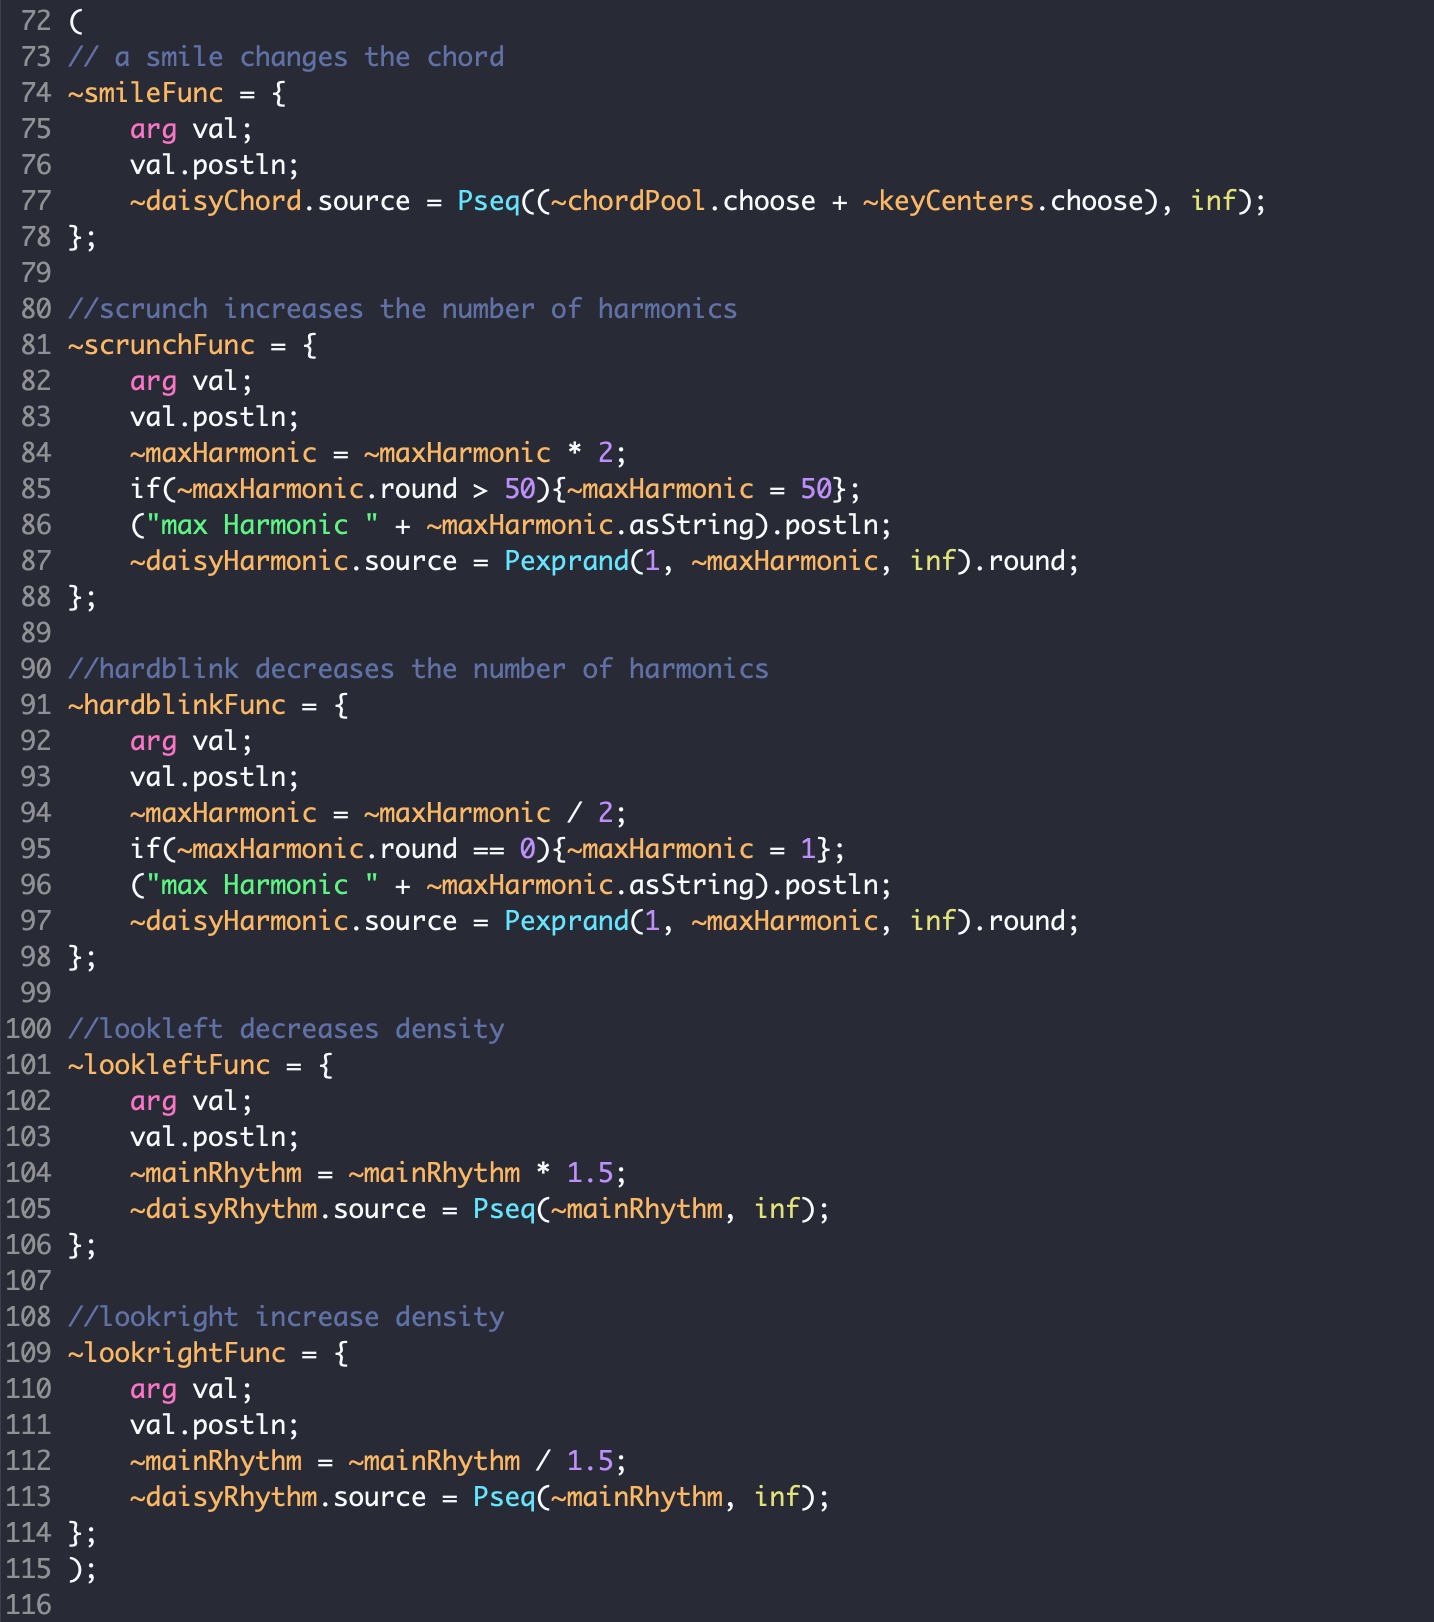
\includegraphics[width=1\columnwidth]{daisypat.png}
	\caption{Facial Expression Controls for Arpeggio Pattern}
	\label{fig:daisypat}
\end{figure}

(Figure~\ref{fig:oscdefs}) shows the facial expression callback functions for a generative arpeggio pattern in SuperCollider. In this particular pattern, a note is chosen randomly from a chord array. Once a note is chosen, the chosen note itself (or one of its overtones) is played through a synthesizer of the user's choice. This process is then repeated over time at a certain density. 

In this example, the following facial expression controls are enabled:

\begin{itemize}
\item A smile expression randomly chooses a new chord from a pre-existing chord bank. 
\item A scrunch expression increases the number of overtones to choose from. 
\item A hard blink expression decreases the number of overtones to choose from. 
\item A look left expression decreases note density with respect to time. 
\item A look right expression increases note density with respect to time.
\end{itemize}




